\documentclass[11pt,letterpaper]{article}

\usepackage[utf8]{inputenc}
\usepackage[T1]{fontenc}
\usepackage[english]{babel}
\usepackage[margin=2.5cm]{geometry}
\usepackage{graphicx}
\usepackage{float}
\usepackage{caption}
\usepackage{booktabs}
\usepackage{tabularx}
\usepackage{array}
\usepackage{enumitem}
\usepackage{xcolor}
\usepackage{listings}
\usepackage{algorithm}
\usepackage{algpseudocode}
\usepackage{amsmath}
\usepackage{amssymb}
\usepackage{etoolbox}
\AtBeginEnvironment{tabularx}{\small}
\usepackage[hidelinks]{hyperref}

\definecolor{codebg}{RGB}{246,246,246}
\definecolor{codecomment}{RGB}{110,110,110}
\definecolor{codekw}{RGB}{0,70,140}
\definecolor{codestr}{RGB}{150,60,0}

\lstset{
  language=Python,
  basicstyle=\ttfamily\small,
  keywordstyle=\color{codekw}\bfseries,
  commentstyle=\color{codecomment}\itshape,
  stringstyle=\color{codestr},
  backgroundcolor=\color{codebg},
  frame=single,
  rulecolor=\color{codebg},
  breaklines=true,
  columns=fullflexible,
  keepspaces=true,
  showstringspaces=false,
  numbers=left,
  numberstyle=\tiny\color{codecomment},
  xleftmargin=1.5em,
  framexleftmargin=1.5em,
  literate={→}{{$\rightarrow$}}1 {á}{{\'a}}1 {é}{{\'e}}1 {ó}{{\'o}}1 {¿}{{?`}}1
}

\newcommand{\code}[1]{\texttt{#1}}
\newcolumntype{L}{>{\raggedright\arraybackslash}X}
\setlength{\parskip}{0.5em}
\setlength{\parindent}{0pt}
\sloppy

% ---------------------------------------------------------------
%  FILL IN: Render link
% ---------------------------------------------------------------
\newcommand{\renderlink}{\url{https://dijkstra-python.onrender.com/}}

\begin{document}

% ===============================================================
%  PRESENTATION SHEET
% ===============================================================
\begin{titlepage}
  \centering
  \vspace*{1cm}
  {\Large Universidad Panamericana\par}
  \vspace{0.4cm}
  {\large Artificial Intelligence for Video Games\par}
  \vspace{2.5cm}
  {\Huge\bfseries Project 2\par}
  \vspace{0.5cm}
  {\LARGE Shortest Path with Bidirectional Dijkstra\par}
  \vspace{3cm}

  {\large\bfseries Team members\par}
  \vspace{0.4cm}
  {\large
  \begin{tabular}{ll}
    % FILL IN: full names and student IDs
    Rodrigo López Gómez {\hspace{3cm}}& ID:  0262146\\[0.3cm]
    Valeria Pérez Maciel{\hspace{3cm}} & ID: 0261983 \\
  \end{tabular}\par}

  \vspace{2.5cm}
  {\large Professor: Alfredo Emmanuel García Falcón{\hspace{6cm}}\par}
  \vfill
  {\large October 2026\par}
\end{titlepage}

\tableofcontents
\newpage

% ===============================================================
\section{Introduction}
% ===============================================================

This project is a web application that lets the user build a directed,
weighted graph visually and find the shortest path between a \emph{start}
node and a \emph{destination} node using the \textbf{bidirectional Dijkstra}
algorithm.

\begin{itemize}[nosep]
  \item \textbf{Algorithm:} \code{dijkstra.py}, written in Python using only
        the standard library (\code{heapq}, \code{itertools}).
  \item \textbf{Backend:} \code{app.py}, a Flask server.
  \item \textbf{Frontend:} \code{index.html}, \code{static/app.js} and
        \code{static/style.css}; the graph is drawn with Cytoscape.js.
  \item \textbf{Deployment:} Render, available at \renderlink.
\end{itemize}

The identifiers of \code{dijkstra.py} are in Spanish: \code{Nodo} (node),
\code{Arista} (edge), \code{Grafo} (graph), \code{peso} (weight),
\code{inicio} (start) and \code{fin} (end). This report keeps the original
names.

\subsection{Relation between \code{dijkstra.py} and \code{app.py}}

\code{dijkstra.py} is the \textbf{base of the algorithm} used by the
application. It was written as a standalone module with its own classes
(\code{Nodo}, \code{Arista}, \code{Grafo}) and can still be executed by
itself.

The graphical interface does not work with those classes directly: the
browser edits a lightweight JSON representation of the graph (nodes, roles,
levels and connections). When the user presses \textbf{SOLVE},
\code{app.py} \textbf{rebuilds that graph as \code{Grafo}/\code{Nodo}
objects} so it is compatible with the algorithm, calls \code{resolver()},
and translates the result (a list of \code{Nodo} objects and a cost) back
into JSON so the interface can highlight the path. Therefore \code{app.py}
acts as the adapter between the graphical part and the algorithm, while the
shortest-path logic lives only in \code{dijkstra.py}.

\begin{center}
\small
\texttt{Browser (app.js)} $\xrightarrow{\text{JSON}}$
\texttt{app.py (Flask)} $\xrightarrow{\texttt{Grafo / Nodo}}$
\texttt{dijkstra.py} $\xrightarrow{\texttt{(path, cost)}}$
\texttt{app.py} $\xrightarrow{\text{JSON}}$ \texttt{Browser}
\end{center}

% ===============================================================
\section{Dijkstra's Algorithm}
% ===============================================================

\subsection{Standard Dijkstra}

Dijkstra's algorithm finds the shortest path from a source node $s$ to every
other node of a graph $G=(V,E)$ whose edge weights are \textbf{non-negative},
$w(u,v)\ge 0$.

The idea is greedy: the algorithm keeps a tentative distance $d[v]$ for every
node and always processes the unvisited node with the smallest tentative
distance. Because no edge has a negative weight, no later path can reach that
node more cheaply, so its distance becomes final.

\begin{algorithm}[H]
\caption{Standard Dijkstra}
\begin{algorithmic}[1]
\Procedure{Dijkstra}{$G, s$}
  \ForAll{$v \in V$}
    \State $d[v] \gets \infty$; \quad $parent[v] \gets \text{null}$
  \EndFor
  \State $d[s] \gets 0$
  \State $Q \gets$ min-priority queue containing $(0, s)$
  \While{$Q$ is not empty}
    \State $(d_u, u) \gets Q.\text{pop\_min}()$
    \If{$u$ already visited} \textbf{continue} \EndIf
    \State mark $u$ as visited
    \ForAll{edge $(u, v)$ with weight $w$}
      \If{$d[u] + w < d[v]$} \Comment{relaxation}
        \State $d[v] \gets d[u] + w$; \quad $parent[v] \gets u$
        \State $Q.\text{push}(d[v], v)$
      \EndIf
    \EndFor
  \EndWhile
  \State \Return $d, parent$
\EndProcedure
\end{algorithmic}
\end{algorithm}

The path to any node $t$ is rebuilt by following $parent$ from $t$ back to
$s$ and reversing the list. Using a binary heap, the complexity is
$O((|V|+|E|)\log|V|)$.

Its weakness is that the search grows like a ``circle'' around the source: to
reach the destination it has to explore every node that is closer than the
destination, in every direction.

\subsection{Bidirectional Dijkstra (used in this project)}

Bidirectional Dijkstra runs \textbf{two Dijkstra searches at the same time}:

\begin{center}
\begin{tabularx}{\textwidth}{lllL}
\toprule
\textbf{Search} & \textbf{Starts at} & \textbf{Follows} & \textbf{Structures} \\
\midrule
Forward ($f$)  & start node       & outgoing edges (\code{aristas})  & \code{dist\_f}, \code{padre\_f}, \code{pq\_f}, \code{vis\_f} \\
Backward ($b$) & destination node & incoming edges (\code{entrantes}), reversed & \code{dist\_b}, \code{padre\_b}, \code{pq\_b}, \code{vis\_b} \\
\bottomrule
\end{tabularx}
\end{center}

Because the graph is directed, the backward search walks the edges ``against
the arrow'': from a node it moves to the \emph{origin} of each incoming edge.
That is why every \code{Nodo} stores both its outgoing and incoming edges.

\textbf{Meeting point.} Every time one search relaxes an edge towards a node
$v$, it also computes $d_{\text{this}}(v) + d_{\text{other}}(v)$. If the
other search has already reached $v$, this is the cost of a complete path
$s \rightsquigarrow v \rightsquigarrow t$. The best such value is kept in
\code{mejor} and its node in \code{encuentro}.

\textbf{Stopping condition.} Let $top_f$ and $top_b$ be the smallest
distances in each queue. Any path not discovered yet must cost at least
$top_f + top_b$, so the algorithm stops when
\[
  top_f + top_b \;\ge\; mejor .
\]

\textbf{Balancing.} On each iteration the search whose queue has the smaller
minimum is expanded, so both ``circles'' grow at a similar rate.

\begin{algorithm}[H]
\caption{Bidirectional Dijkstra (\code{dijkstra\_bidireccional})}
\begin{algorithmic}[1]
\Procedure{BidirectionalDijkstra}{$G, s, t$}
  \If{$s = t$} \Return $([s], 0)$ \EndIf
  \State $d_f[\cdot], d_b[\cdot] \gets \infty$; \quad $d_f[s] \gets 0$; \quad $d_b[t] \gets 0$
  \State $Q_f \gets \{(0, s)\}$; \quad $Q_b \gets \{(0, t)\}$
  \State $mejor \gets \infty$; \quad $encuentro \gets \text{null}$
  \While{$Q_f$ and $Q_b$ are not empty}
    \If{$top(Q_f) + top(Q_b) \ge mejor$} \textbf{break} \EndIf
    \If{$top(Q_f) \le top(Q_b)$}
      \State \Call{Expand}{$Q_f, d_f, d_b$, outgoing edges}
    \Else
      \State \Call{Expand}{$Q_b, d_b, d_f$, incoming edges}
    \EndIf
  \EndWhile
  \If{$encuentro = \text{null}$} \Return $(\text{null}, \infty)$ \EndIf
  \State $path \gets$ reverse(follow $parent_f$ from $encuentro$)
  \State append (follow $parent_b$ from $parent_b[encuentro]$) to $path$
  \State \Return $(path, mejor)$
\EndProcedure
\Statex
\Procedure{Expand}{$Q, d, d_{other}$, edges}
  \State $(d_u, u) \gets Q.\text{pop\_min}()$
  \If{$u$ already visited} \Return \EndIf
  \State mark $u$ as visited
  \ForAll{neighbor $v$ of $u$ through an edge of weight $w$}
    \State $new \gets d_u + w$
    \If{$new < d[v]$}
      \State $d[v] \gets new$; \quad $parent[v] \gets u$; \quad $Q.\text{push}(new, v)$
    \EndIf
    \If{$new + d_{other}[v] < mejor$}
      \State $mejor \gets new + d_{other}[v]$; \quad $encuentro \gets v$
    \EndIf
  \EndFor
\EndProcedure
\end{algorithmic}
\end{algorithm}

The path is rebuilt in two halves: from the start to the meeting node
following \code{padre\_f} (and reversing), and from the meeting node to the
destination following \code{padre\_b}, which already points towards the
destination.

The worst-case complexity is the same as standard Dijkstra,
$O((|V|+|E|)\log|V|)$, but in practice each search only covers about half of
the distance, so two small ``circles'' explore far fewer nodes than one big
circle. If there is no path, the queues run out without the searches meeting
and the method returns \code{(None, inf)}.

% ===============================================================
\section{Data Structures, Classes, Methods and Attributes}
% ===============================================================

\subsection{\code{dijkstra.py} --- the algorithm}

Only the elements that the application uses are described.

\subsubsection*{Class \code{Nodo} (node)}

\begin{tabularx}{\textwidth}{llL}
\toprule
\textbf{Attribute} & \textbf{Type} & \textbf{Description} \\
\midrule
\code{nombre}    & \code{str}           & Name of the node (unique in the app). \\
\code{aristas}   & \code{list[Arista]}  & Outgoing edges; used by the forward search. \\
\code{entrantes} & \code{list[Arista]}  & Incoming edges; used by the backward search. \\
\bottomrule
\end{tabularx}

\begin{tabularx}{\textwidth}{lL}
\toprule
\textbf{Method} & \textbf{Description} \\
\midrule
\code{\_\_init\_\_(nombre)} & Creates the node with empty edge lists. \\
\code{\_\_repr\_\_()}       & Text representation, e.g.\ \code{Nodo(A)}. \\
\bottomrule
\end{tabularx}

\subsubsection*{Class \code{Arista} (directed, weighted edge)}

The application never creates it directly; it is created inside
\code{Grafo.agregar\_arista}.

\begin{tabularx}{\textwidth}{llL}
\toprule
\textbf{Attribute} & \textbf{Type} & \textbf{Description} \\
\midrule
\code{origen}  & \code{Nodo}               & Node where the edge starts. \\
\code{destino} & \code{Nodo}               & Node where the edge ends. \\
\code{peso}    & \code{int} / \code{float} & Weight (cost) of the edge, must be $\ge 0$. \\
\bottomrule
\end{tabularx}

\begin{tabularx}{\textwidth}{lL}
\toprule
\textbf{Method} & \textbf{Description} \\
\midrule
\code{\_\_init\_\_(origen, destino, peso)} & Creates the edge; raises \code{ValueError} if the weight is negative, because Dijkstra does not support negative weights. \\
\code{\_\_repr\_\_()} & Text representation, e.g.\ \code{A -> B (4)}. \\
\bottomrule
\end{tabularx}

\subsubsection*{Class \code{Grafo} (graph and algorithm)}

\begin{tabularx}{\textwidth}{llL}
\toprule
\textbf{Attribute} & \textbf{Type} & \textbf{Description} \\
\midrule
\code{nodos}  & \code{list[Nodo]}      & Every node in the graph. \\
\code{inicio} & \code{Nodo} or \code{None} & Start node. \\
\code{fin}    & \code{Nodo} or \code{None} & Destination node. \\
\bottomrule
\end{tabularx}

\begin{tabularx}{\textwidth}{>{\raggedright\arraybackslash}p{5.2cm}L}
\toprule
\textbf{Method} & \textbf{Description} \\
\midrule
\code{agregar\_nodo(nodo)} & Adds the node if it is not already in the graph and returns it. \\
\code{agregar\_arista(origen, destino, peso)} & Adds both nodes if needed, creates the \code{Arista}, appends it to \code{origen.aristas} and to \code{destino.entrantes}, and returns it. \\
\code{set\_inicio(nodo)}, \code{set\_fin(nodo)} & Set the start / destination node; raise \code{ValueError} if the node does not belong to the graph. \\
\code{resolver()} & Checks that start and destination are set and returns \code{dijkstra\_bidireccional(inicio, fin)}, i.e.\ \code{(path, cost)}. \\
\code{dijkstra\_bidireccional(}\allowbreak\code{origen, destino)} & Runs the bidirectional search (Section 2.2). Returns \code{(list[Nodo], cost)} or \code{(None, inf)}. \\
\code{\_expandir(pq, dist, padre, visitados, dist\_otro, adelante, mejor, encuentro, contador)} & One step of one search: pops the closest node, marks it visited, relaxes its edges (outgoing if \code{adelante} is \code{True}, incoming otherwise) and updates \code{mejor}/\code{encuentro} when it touches the other search. Returns the new \code{(mejor, encuentro)}. \\
\bottomrule
\end{tabularx}

\subsubsection*{Data structures inside \code{dijkstra\_bidireccional}}

\begin{tabularx}{\textwidth}{>{\raggedright\arraybackslash}p{3cm}>{\raggedright\arraybackslash}p{3.8cm}L}
\toprule
\textbf{Name} & \textbf{Structure} & \textbf{Purpose} \\
\midrule
\code{dist\_f}, \code{dist\_b} & \code{dict[Nodo, float]} & Best known distance from the start / to the destination. \\
\code{padre\_f}, \code{padre\_b} & \code{dict[Nodo, Nodo]} & Previous node in each search; used to rebuild the path. \\
\code{vis\_f}, \code{vis\_b} & \code{set[Nodo]} & Nodes whose distance is already final. \\
\code{pq\_f}, \code{pq\_b} & \code{list} used as a min-heap (\code{heapq}) & Priority queues with tuples \code{(distance, counter, node)}. \\
\code{contador} & \code{itertools.count()} & Tie-breaker: when two distances are equal the heap compares this number instead of the \code{Nodo} objects, which are not comparable. \\
\code{mejor} & \code{float} & Cost of the best complete path found so far. \\
\code{encuentro} & \code{Nodo} & Meeting node of that best path. \\
\bottomrule
\end{tabularx}

\subsection{\code{app.py} --- Flask backend and adapter}

\subsubsection*{Graph state}

Each browser session has its own graph, kept in memory as plain dictionaries
that can be sent as JSON.

\begin{tabularx}{\textwidth}{>{\raggedright\arraybackslash}p{3.2cm}L}
\toprule
\textbf{Structure} & \textbf{Description} \\
\midrule
\code{\_GRAPH\_STATES} & \code{dict[graph\_id, state]}: all graphs, keyed by an id stored in the Flask session cookie. \\
\code{\_STATE\_LOCK} & \code{threading.RLock} that protects the states from concurrent requests. \\
\code{\_MAX\_NODES} & Limit of 40 nodes per graph. \\
state & \code{\{"nodes": [...], "max\_level": int, "solution": dict | None\}} \\
node & \code{\{"id", "name", "role", "level", "edges"\}}. \code{role} is \code{"start"}, \code{"finish"} or \code{""}; \code{level} is the column where the node is drawn (start = 0, destination = last). \\
edge & \code{\{"to": node\_id, "weight": number\}}, stored in the source node. \\
solution & \code{\{"reachable", "pathIds", "pathNames", "cost", "message"\}}. \\
\bottomrule
\end{tabularx}

\subsubsection*{Helper functions}

\begin{tabularx}{\textwidth}{>{\raggedright\arraybackslash}p{5.2cm}L}
\toprule
\textbf{Function} & \textbf{Description} \\
\midrule
\code{\_new\_node(name, role, level)} & Creates a node dictionary with a random id. \\
\code{\_initial\_state()} & New graph with \code{A} (start) and \code{B} (destination). \\
\code{\_state()} & Returns the graph of the current session, creating it if needed. \\
\code{\_state\_response()}, \code{\_error()} & Build the JSON responses (state, plus an error message when applicable). \\
\code{\_find\_node(state, id)} & Looks up a node by id. \\
\code{\_invalidate\_solution(state)} & Clears the previous result whenever the graph changes. \\
\code{\_normalise\_levels(state)} & Keeps start at level 0, regular nodes at level $\ge 1$ and the destination one level after the last regular node. \\
\code{\_parse\_weight(value)} & Validates that a weight is a finite number $\ge 0$. \\
\code{\_next\_name(state)} & Next free name: \code{A}\ldots\code{Z}, then \code{N1}, \code{N2}, \ldots \\
\code{\_reassign\_endpoint\_}\allowbreak\code{if\_needed()} & If the start or destination is deleted, promotes another node so both always exist. \\
\bottomrule
\end{tabularx}

\subsubsection*{HTTP endpoints}

\begin{tabularx}{\textwidth}{>{\raggedright\arraybackslash}p{6.3cm}L}
\toprule
\textbf{Route} & \textbf{Description} \\
\midrule
\code{GET /} & Serves \code{index.html}. \\
\code{GET /api/state} & Returns the current graph. \\
\code{POST /api/nodes} & Adds a node. \\
\code{PATCH /api/nodes/<id>} & Renames a node or changes its role. \\
\code{DELETE /api/nodes/<id>} & Deletes a node and every edge pointing to it. \\
\code{POST /api/nodes/<id>/level} & Moves a regular node one level left or right. \\
\code{POST /api/nodes/<id>/edges} & Adds (or updates) a connection \code{\{to, weight\}}. \\
\code{DELETE /api/nodes/<id>/edges/<to>} & Removes a connection. \\
\code{POST /api/solve} & Builds the \code{Grafo} and runs the algorithm. \\
\code{GET /health} & Health check used by Render. \\
\bottomrule
\end{tabularx}

\subsubsection*{Connection with the algorithm: \code{solve()}}

This is where the interface and \code{dijkstra.py} meet. After validating
that names are complete and unique and that there is exactly one start and
one destination, \code{solve()} rebuilds the graph with the classes of
\code{dijkstra.py}:

\begin{lstlisting}
graph = Grafo()
node_objects = {node["id"]: Nodo(node["name"].strip()) for node in nodes}
for node in nodes:
    graph.agregar_nodo(node_objects[node["id"]])
for node in nodes:
    for edge in node["edges"]:
        destination = _find_node(state, edge["to"])
        graph.agregar_arista(node_objects[node["id"]],
                             node_objects[destination["id"]],
                             _parse_weight(edge["weight"]))
graph.set_inicio(node_objects[starts[0]["id"]])
graph.set_fin(node_objects[finishes[0]["id"]])
path, cost = graph.resolver()
\end{lstlisting}

The resulting list of \code{Nodo} objects is converted back to names and ids
(\code{pathNames}, \code{pathIds}) and stored in \code{state["solution"]}.

\subsection{\code{static/app.js} --- frontend}

\begin{itemize}[nosep]
  \item \code{state}: local copy of the graph returned by the server; every
        action sends a request and redraws using the new state.
  \item \code{api(path, method, body)}: sends requests to the backend and
        shows errors in a toast message.
  \item \code{card(node)}: builds each node card (name, role, connections and
        the form to add connections).
  \item \code{drawGraph()}: draws the graph with Cytoscape.js, placing each
        node in the column of its \code{level}. After solving, the path is
        drawn with thick lines and the rest of the graph is faded.
  \item \code{panels()}: shows the level-move panel of the selected node and
        the result card (total cost and path).
\end{itemize}

% ===============================================================
\section{Instructions to Create a Graph}
% ===============================================================

The page has three areas: the \textbf{node cards} (top), the \textbf{graph}
drawing (bottom) and the \textbf{SOLVE} button (bottom right).

\begin{enumerate}
  \item \textbf{Initial graph.} The page starts with node \code{A}
        (\textbf{Start}, green border) and node \code{B}
        (\textbf{Destination}, red border).
  \item \textbf{Add nodes.} Click the \textbf{+} card at the end of the row.
        Each new node receives the next free name (\code{C}, \code{D},
        \ldots). Up to 40 nodes are allowed.
  \item \textbf{Rename a node.} Edit the text field of its card (at most 24
        characters; names must be unique).
  \item \textbf{Change the start or destination.} In the dropdown of a
        regular node choose \textbf{Start} or \textbf{Destination}; the
        previous one becomes a regular node.
  \item \textbf{Add a connection (directed edge).} At the bottom of the
        \emph{source} node's card select the target node, type the weight
        (a number $\ge 0$) and press \textbf{+}. The connection appears as a
        chip ``\code{Target $\cdot$ weight}''. Adding the same connection
        again only updates its weight. For a two-way connection, add it from
        both cards.
  \item \textbf{Remove a connection.} Click the \textbf{$\times$} on its chip.
  \item \textbf{Delete a node.} Click the \textbf{$\times$} in the card
        header (only when the graph has more than two nodes). Its connections
        are deleted as well.
  \item \textbf{Reorder the drawing (optional).} Click a regular node in the
        graph and use \textbf{$\leftarrow$ Left / Right $\rightarrow$} to move
        it to another column. This only changes the drawing, not the result.
  \item \textbf{Solve.} Press \textbf{SOLVE}. The result card shows the
        \textbf{total cost} and the \textbf{path} (e.g.\
        \code{A $\rightarrow$ C $\rightarrow$ D $\rightarrow$ B}) and the
        graph highlights it. If no path exists, it shows ``No route found''.
        Any later change to the graph clears the result.
\end{enumerate}

% ===============================================================
\section{Instructions to Run the Code}
% ===============================================================

\textbf{Running the project locally is not required:} the application is
deployed on Render and can be used directly at:

\begin{center}
  \Large \renderlink
\end{center}

\subsection*{Requirements}
\begin{itemize}[nosep]
  \item Python 3.12 or newer.
  \item The packages listed in \code{requirements.txt} (Flask and Gunicorn).
  \item Internet connection in the browser (Cytoscape.js is loaded from a CDN).
\end{itemize}

\subsection*{Steps}

\begin{lstlisting}[language=bash,numbers=none]
# Create and activate a virtual environment
python3 -m venv venv
source venv/bin/activate        # Windows: venv\Scripts\activate

# Install the dependencies
pip install -r requirements.txt

# Run the application
python app.py
\end{lstlisting}

Then open \url{http://localhost:5000} in the browser. The address
\url{http://localhost:5000/health} should return \code{\{"status":"ok"\}}.

\subsection*{Options}
\begin{itemize}
  \item \textbf{Different port:} \code{PORT=8000 python app.py}
  \item \textbf{Keep the session between restarts:}
        \code{SECRET\_KEY=any-fixed-text python app.py}. Otherwise a new key
        is generated on each start and the browser gets a new, empty graph.
  \item \textbf{Run it as on Render (Gunicorn):}
        \code{gunicorn -w 1 -b 0.0.0.0:5000 app:app}. A single worker
        (\code{-w 1}) must be used because graphs are kept in memory; with
        several workers each one would hold a different copy.
\end{itemize}

\subsection*{Running only the algorithm}

\code{dijkstra.py} can also be executed on its own and needs no
dependencies:

\begin{lstlisting}[language=bash,numbers=none]
python dijkstra.py
\end{lstlisting}

Its example builds a $20\times20$ grid with \textbf{400 nodes}
(\code{N0} \ldots\ \code{N399}). Each node has a directed edge to the right
and one downward, with weights between 1 and 9, which gives 760 edges. The
program finds the shortest path from the top-left corner (\code{N0}) to the
bottom-right corner (\code{N399}) and prints:

\begin{lstlisting}[language={},numbers=none]
Nodos en el grafo: 400
Camino (39 nodos): N0 -> N1 -> N2 -> N3 -> N4 -> N24 -> N44 -> N45 ->
  N65 -> N85 -> N86 -> N106 -> N126 -> N127 -> N147 -> N167 -> N168 ->
  N169 -> N189 -> N190 -> N191 -> N192 -> N193 -> N213 -> N233 -> N234 ->
  N254 -> N274 -> N275 -> N295 -> N315 -> N316 -> N336 -> N356 -> N357 ->
  N377 -> N397 -> N398 -> N399
Costo total: 106
\end{lstlisting}

That is, the number of nodes in the graph, the path (39 nodes) and its total
cost (106). The result was cross-checked with a standard Dijkstra over the
same graph, which gives the same cost.

% ===============================================================
\section{Execution Results}
% ===============================================================

The following screenshots show the program running: the creation of the
graph in the node cards, the drawing generated from them and the result of
the algorithm after pressing \textbf{SOLVE}. The shortest path is drawn with
thick lines and the nodes and edges that are not part of it are faded.

\begin{figure}[H]
  \centering
  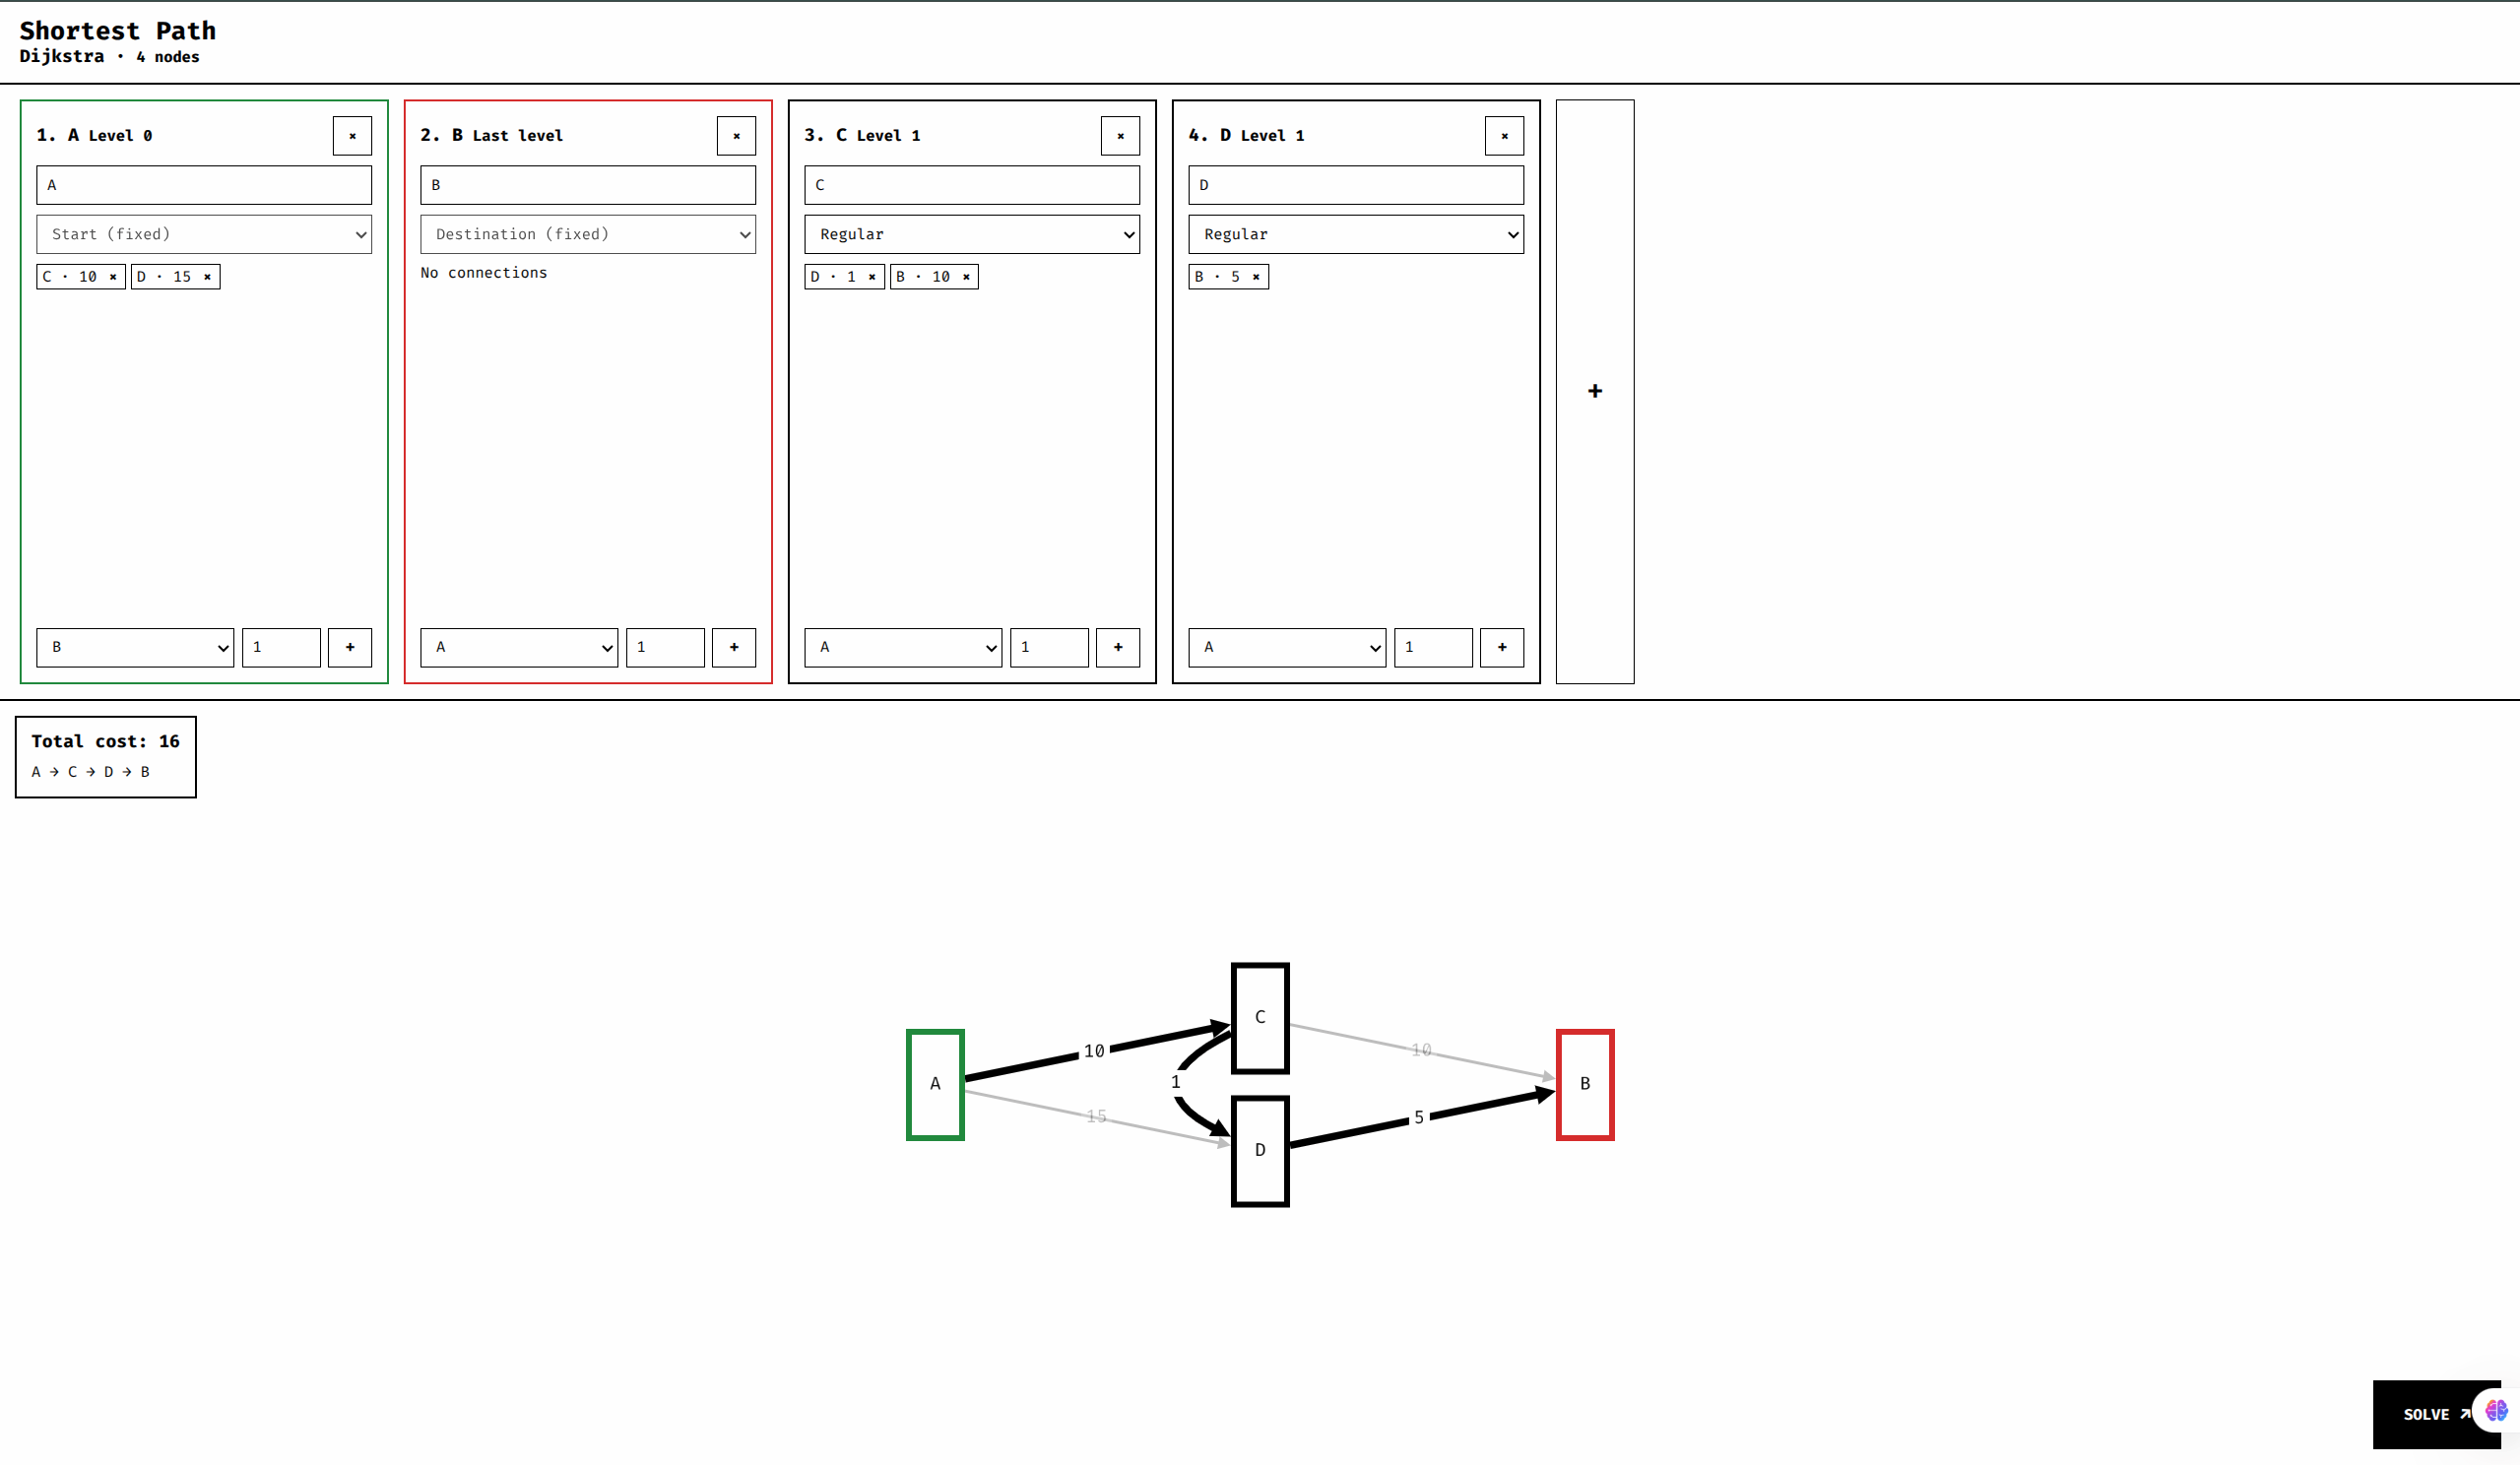
\includegraphics[width=0.7\textwidth]{execution2.png}
  \caption{Graph with 4 nodes. From \code{A} the direct edges cost 10
  (to \code{C}) and 15 (to \code{D}), and from \code{C} going to \code{B}
  directly costs 10. The algorithm finds that going through \code{D}
  is cheaper: \code{A $\rightarrow$ C $\rightarrow$ D $\rightarrow$ B} with a
  total cost of $10+1+5=16$ (the alternatives cost 20).}
  \label{fig:exec2}
\end{figure}

\begin{figure}[H]
  \centering
  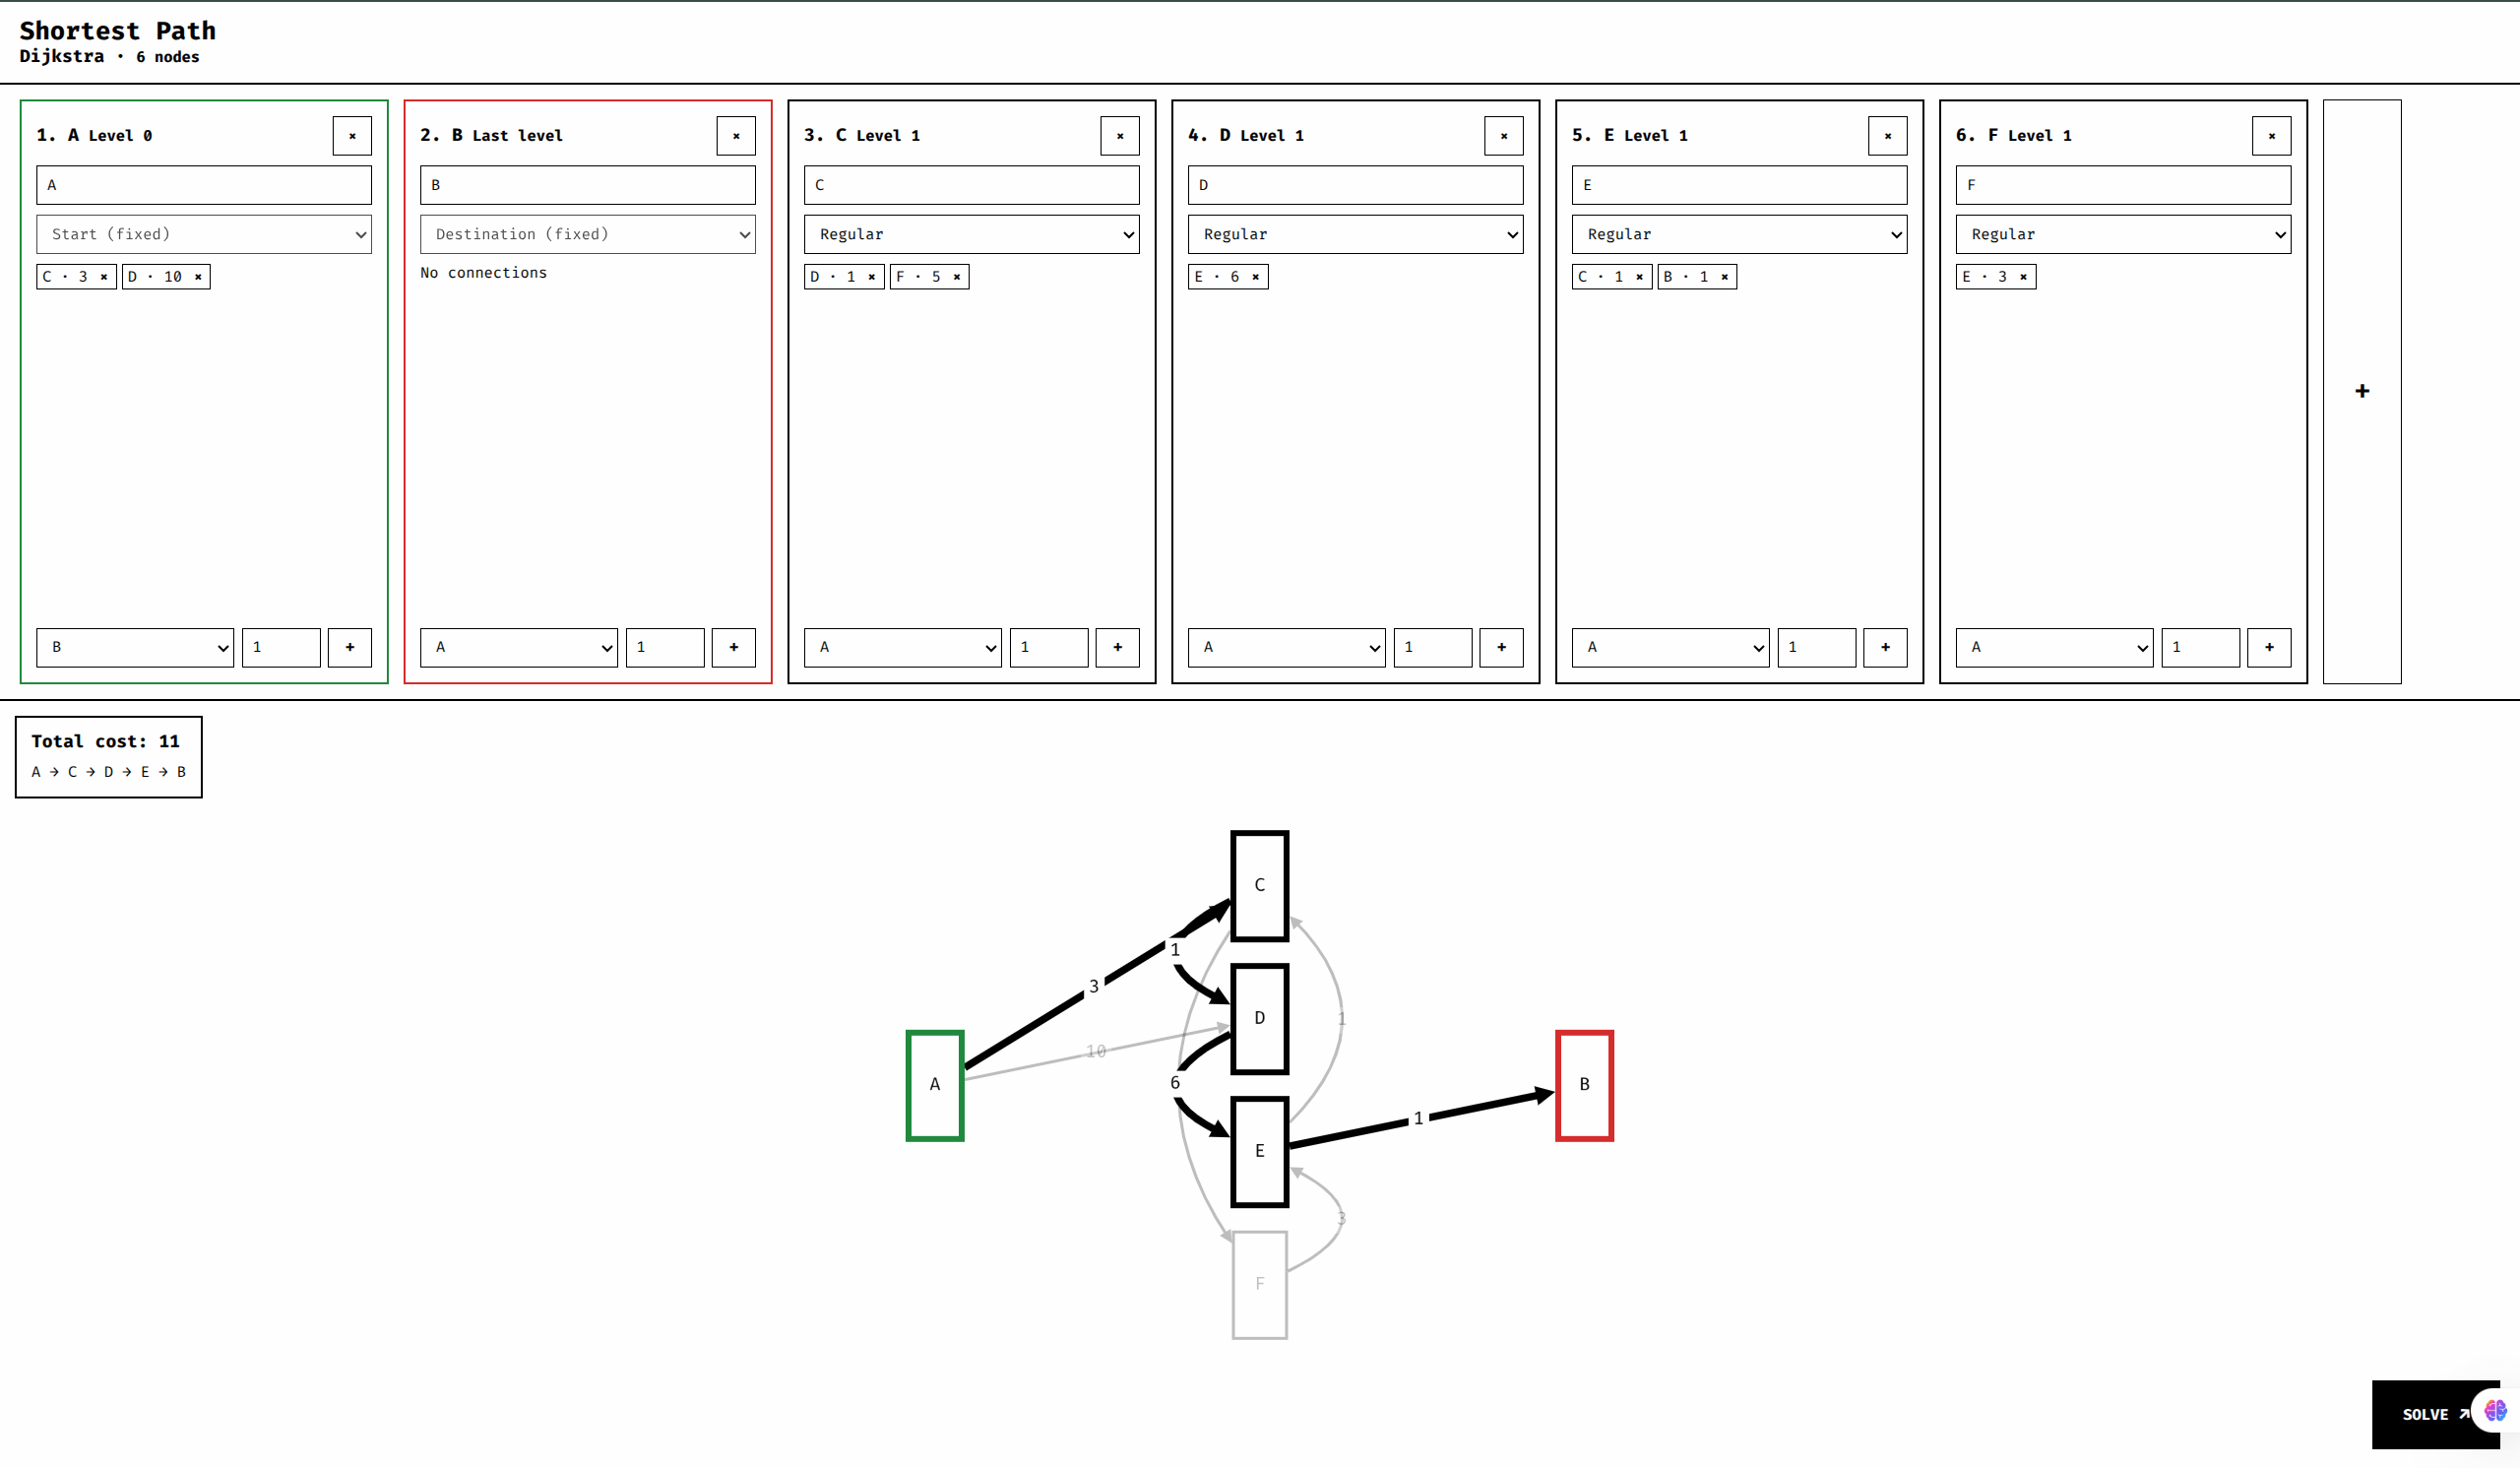
\includegraphics[width=0.7\textwidth]{execution1.png}
  \caption{Graph with 6 nodes, including a node (\code{F}) that is not on
  the optimal route. Result: \code{A $\rightarrow$ C $\rightarrow$ D
  $\rightarrow$ E $\rightarrow$ B} with a total cost of $3+1+6+1=11$; the
  direct edge \code{A $\rightarrow$ D} (10) is not used.}
  \label{fig:exec1}
\end{figure}

\begin{figure}[H]
  \centering
  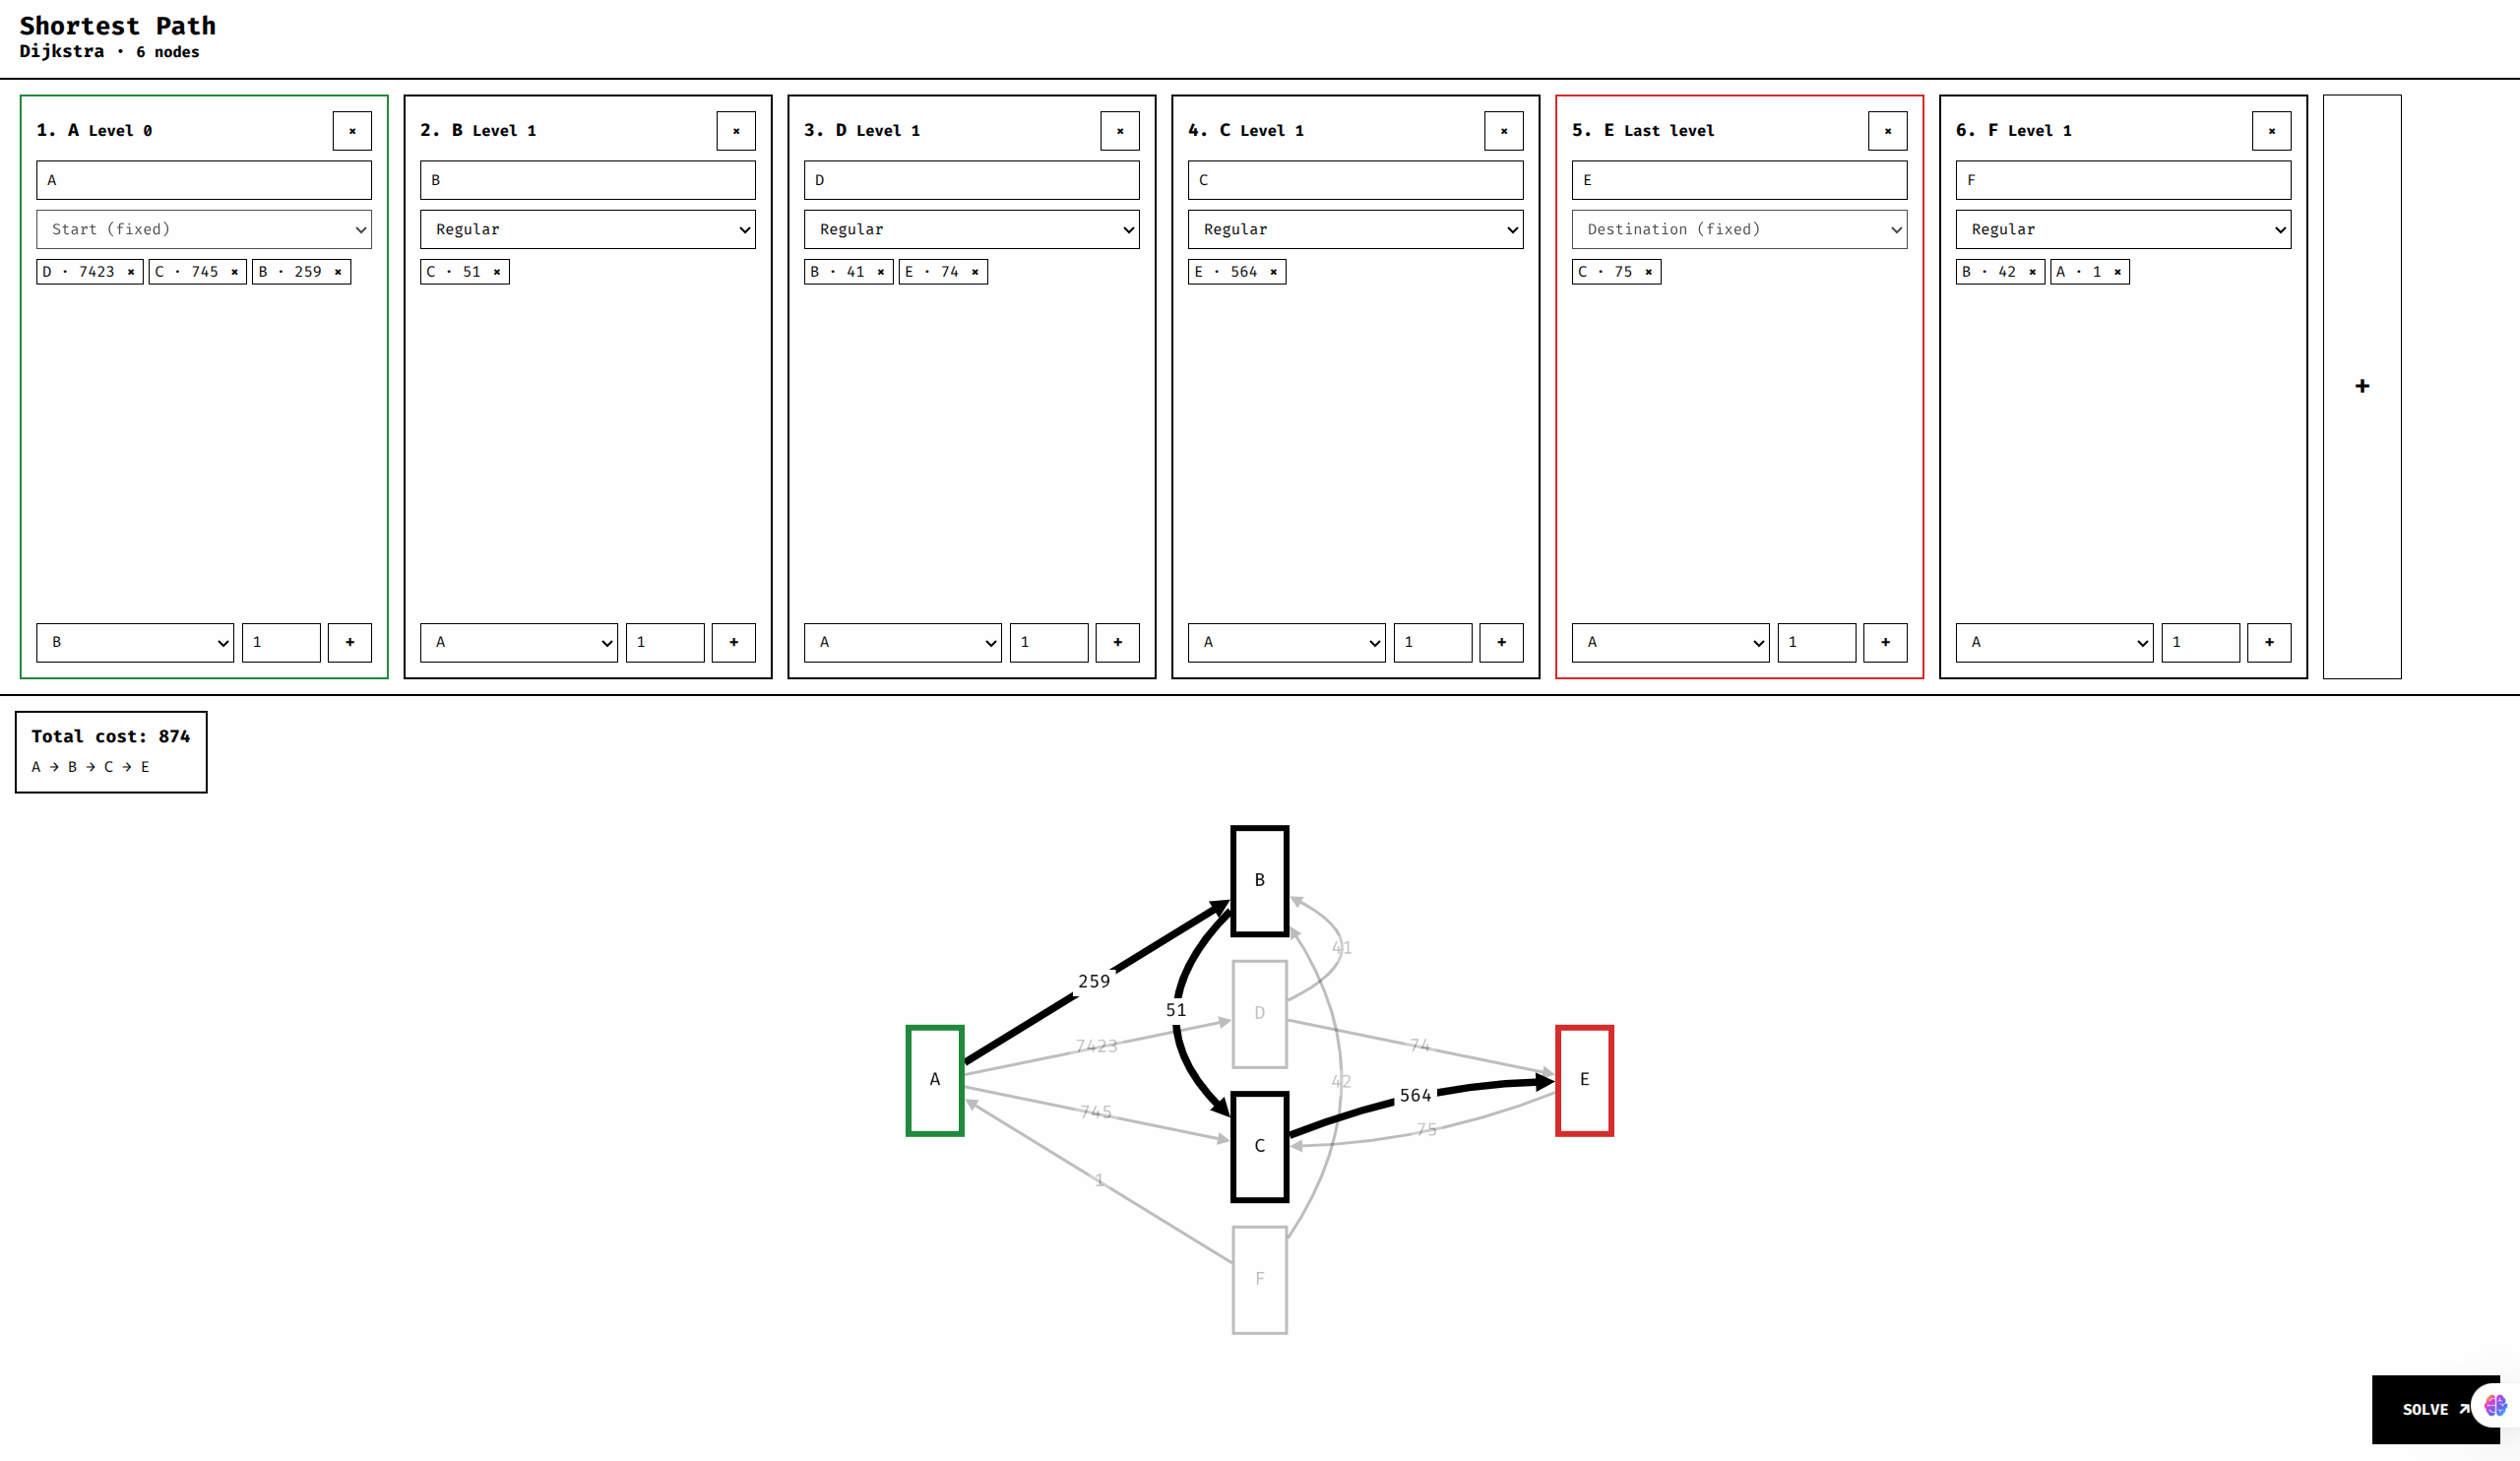
\includegraphics[width=0.7\textwidth]{execution3.png}
  \caption{Graph with 6 nodes, large weights and edges that go back to the
  start (\code{F $\rightarrow$ A}) and from the destination
  (\code{E $\rightarrow$ C}). The destination was changed to \code{E}.
  Result: \code{A $\rightarrow$ B $\rightarrow$ C $\rightarrow$ E} with a
  total cost of $259+51+564=874$, cheaper than \code{A $\rightarrow$ C
  $\rightarrow$ E} (1309) or any route through \code{D} (7423 for the
  first edge alone).}
  \label{fig:exec3}
\end{figure}

% ===============================================================
\section{Conclusions}
% ===============================================================

% FILL IN: each team member's conclusion

\subsection*{Rodrigo López Gómez}
For me, this project was a good opportunity to understand how an algorithm that we learn about in class can actually be used to create something functional. At first, the main goal was to implement Dijkstra’s algorithm and make it find the shortest path between nodes, but as we worked on the project, I realized that there was more to it than just making the algorithm work. We also had to think about how someone would use the application and how all the different parts would work together.

When we decided how to build the interface, we went with HTML and CSS, using a little bit of JavaScript for some interactions. We wanted to keep things simple and focus on making the application easy to understand and use without adding unnecessary complexity. For the backend, we used Python with Flask to connect the interface to the algorithm. Instead of making everything part of one large program, we kept the Dijkstra algorithm in its own file and used it like a small API. This way, the interface could send the graph information to the server, the algorithm could calculate the shortest path, and the result could be returned to the user. I think this was one of the most interesting parts of the project because it helped me understand better how the frontend and backend communicate in a real application.

We also deployed the application on Render, which was an important step because it allowed us to make the project available online instead of only running it on our own computers. This made the project feel more complete, since we were not just submitting code that worked locally, but an application that could actually be accessed and used. It also helped me understand that deploying a project is another part of software development that requires attention, just like implementing the features themselves.

Overall, I feel that this project helped me connect what we learn in class with the process of building a real application. I learned that developing software involves more than solving the main problem; it also requires making decisions about the interface, organizing the code, connecting different technologies, and making sure everything works together. I also learned that keeping things simple can be a good decision when it helps make the project easier to understand and maintain. For me, the most satisfying part was seeing how the Dijkstra algorithm could become part of a complete application instead of remaining just a concept in a programming assignment.

\subsection*{Valeria Pérez Maciel}
For me, the most interesting part of this project was the algorithm in \code{dijkstra.py}. We already knew how standard Dijkstra works from class, but implementing the bidirectional version made us understand it much more deeply. It is not enough to run the same search twice: both searches have to share information to know when they meet, and the program has to know exactly when it is safe to stop. Working out why the condition $top_f + top_b \ge mejor$ guarantees that no better path can still appear was one of the moments where the theory really made sense to me.

The fact that the graph is directed also made us think about details that are easy to overlook. The backward search cannot use the same edges as the forward one, because it has to walk ``against the arrow'', so we decided that every \code{Nodo} should store both its outgoing edges (\code{aristas}) and its incoming edges (\code{entrantes}). Rebuilding the final path in two halves, one with \code{padre\_f} and one with \code{padre\_b}, also required care, since a small mistake there would return a path with a repeated or missing node. We also had to solve practical problems, such as the heap trying to compare two \code{Nodo} objects when their distances were equal, which we fixed by adding a counter as a tie-breaker. Small decisions like this, or rejecting negative weights in \code{Arista}, showed us that a correct algorithm also depends on handling these cases properly.

Another decision that helped us was keeping \code{dijkstra.py} as an independent module and testing it on its own before connecting it to the interface. We ran it with a $20\times20$ grid of 400 nodes and compared the result with a standard Dijkstra, which gave us confidence that the bidirectional version was correct. Once it worked, connecting it to \code{app.py} was much easier, because the backend only had to rebuild the graph with our classes and call \code{resolver()}.

What I take away from this project is a much clearer understanding of how a pathfinding algorithm works internally, and why bidirectional Dijkstra is useful in areas like video games, where finding routes quickly matters: instead of one large search that grows in every direction, two smaller searches meet in the middle and explore far fewer nodes. I also learned the importance of testing each part separately and paying attention to edge cases, because that is what turns an idea from class into a program that actually works. I am satisfied with the final result, an application where anyone can build their own graph and see the shortest path highlighted.


\end{document}
